\section{HMM and sparsity}
When a \gls{hmm} is used to model real world processes, it is often the case that the transition matrix becomes sparse due to the nature of the process.
For example, in human trait recognition, a \gls{hmm} can be used to model the motion of a particular person while he walks.
If focusing on the lower part of the body, consider one state that represents the longest gap between the two feet while walking, where the right foot is in front. It is natural that this state cannot directly lead to the opposite state where the left foot is in front. There has to be a number of intermediate states to represent a more fluid movement, and hence it makes sense to use a sparse model.

When building a system to recognize handwritten text, a \gls{hmm} can be used to model the initial probability of specific letters in a word as well as the probability of seeing a given letter based on the letter the precedes it.
In the English language (and possible many other languages), some letter combinations happens so rarely that it can be neglected.
An example of this can be seen in \figref{fig:ocr-transitions}, which was made from an analysis of 6020 handwritten words provided by Rob Kassel at MIT Spoken Language Systems Group.

\begin{figure}
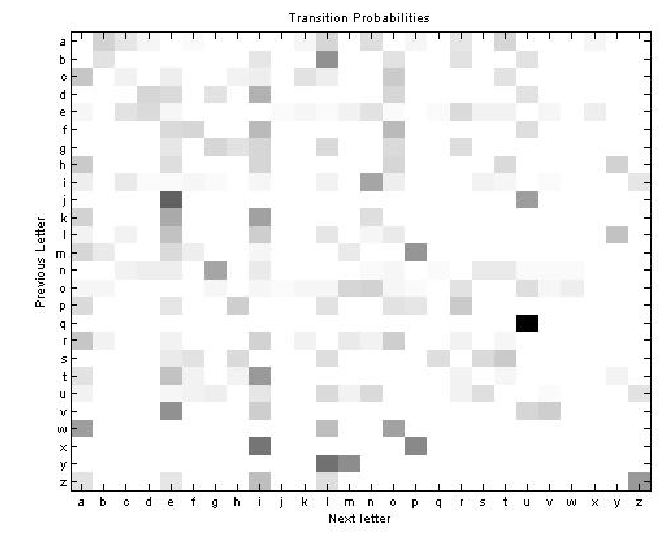
\includegraphics[scale=0.4]{pictures/ocr-transitions.png}
\label{ocr-transitions}
\caption{The transition probabilities between two letters in an English word. White colour denotes a probability of 0 while black denotes a probability of 1.}
\end{figure}
